% Copyright 2026 Torbjörn E. M. Nordling
% SPDX-License-Identifier: Apache-2.0
% frame-hysteresis.tex — Up and down: hysteresis (12:30–14:00)
% Article §3.4: \StartDuty, \StopDuty, \NegStartDuty, \NegStopDuty,
% \StartStopRatio, \DownZeroDelayD, \DownUpRatio.
\begin{frame}{Step 4: up and back down --- hysteresis}{P3 fails}
  \footnotesize
  \begin{columns}[T]
    \column{0.58\textwidth}
    \centering
    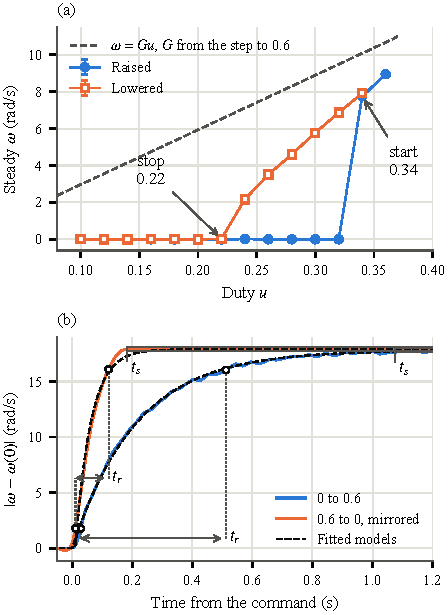
\includegraphics[width=\linewidth, height=0.74\textheight, keepaspectratio]{fig-hysteresis.pdf}
    \column{0.4\textwidth}
    \scriptsize
    \begin{itemize}\setlength{\itemsep}{3pt}
      \item Starts at duty \StartDuty{} going up, stops at \StopDuty{} going down (negative: $-\NegStartDuty$ and $-\NegStopDuty$).
      \item The stop $0.6 \to 0$ has a $\tau$ \alert{\StartStopRatio{} times shorter} than the start, and a dead time of $\DownZeroDelayD$\,ms.
      \item $1.0 \to 0.6$ is \alert{\DownUpRatio{} times slower} than $0.6 \to 1.0$.
    \end{itemize}
    \textbf{Causes:} static friction exceeds Coulomb friction; duty 0 short-circuits the motor, which brakes it; at positive duty the PWM cannot reverse the current, so only friction slows the wheel.
  \end{columns}
\end{frame}
